\section{Fundamentals}
\label{sec:fundamentals}
	
	\subsection{Soil Parameters}
	\label{ssec:soil-parameters}
	
		Let $A$ be any substance in a given soil sample with volume $V\in(0,\infty)$ and let $n_A\in(0,\infty)$ be the amount of $A$ in the sample.
		Then the molar concentration $c_A$ is given by
		\[
			c_A \define \frac{n_A}{V}
		\]
		Now let $c_0$ be the molar concentration of this whole sample.
		We define the amount-of-substance fraction (ASF) $p_A$ of $A$ as 
		\[
			p_A \define 100\%\cdot\frac{c_A}{c_0}
		\]

		In this elaboration we concentrate on three main soil parameters that are given by existing NIRS-measurements.
		The first two parameters $p_\m{SOC}$ and $p_\m{N}$ are ASFs relating to soil organic carbon (SOC) and nitrogen in the soil sample.
		SOC is the carbon in this sample which is bound in an organic compound.
		The third parameter is the $\m{pH}$-value that is used to specify the acidity or basicity of an aqueous solution.
		It is based on the concentration of hydronium ions $c_\m{H_3O^+}$.
		\[
			\m{pH} \define -\log_{10} c_\m{H_3O^+} = -\frac{\ln c_\m{H_3O^+}}{\ln 10}
		\]
	
	% subsection soil-parameters

	\subsection{NIRS}
	\label{ssec:nirs}
	
		In NIRS one uses electromagnetic waves, also known as light, with a wavelength from $780\unit{nm}$ to $3000\unit{nm}$.
		This area is called the near infrared region and is the most energetic one of the infrared light.
		% Quelle: https://de.wikipedia.org/wiki/Nahes_Infrarot

		An emitted light wave with a certain wavelength $\lambda$ can interact with a soil sample in three ways.
		It can be reflected, absorbed or transmitted.
		For most soil samples measuring the transmittance of light waves is not sensible because thickness of these samples varies.
		So the measurement of the spectrum is reduced to the reflectance since absorptance cannot be directly determined.
		% Quelle: Tutorial

		The amount of reflection divides again in specular and diffuse reflection.
		For our purpose only the diffuse part shall be considered.
		This is the one which penetrates the soil sample most.
		As a consequence, diffuse reflected light is scattered among the hemisphere and contains information about the used soil sample.
		For a more detailed view on this topic please refer to [Tutorial].
		% Quelle: Tutorial

		The reflectance $\varrho(\lambda)$ referring to a wavelength $\lambda$ of a light wave of a surface is given by the amount of radiation power $P_\m{r}$ that is reflected from a surface divided by the initial power $P_0$ of this light wave.
		\[
			\varrho(\lambda) \define \frac{P_\m{r}}{P_0}
		\]
		This function $\varrho$ is then called (in our case) the near infrared spectrum of the soil sample.

		Absorptance itself originates from the existence of vibrational modes in molecules.
		A photon with a wavelength $\lambda$ can only be absorbed if the appropriate frequency $f$ exactly matches a multiple of the transition energy of the bond or group that vibrates.
		This is why the spectra of soil samples are formed of overtones and combinations bands.
		% Quelle: Tutorial, https://en.wikipedia.org/wiki/Infrared_spectroscopy

		As a matter of fact it is because of the similarity of diffuse reflected and transmitted light that we can use the Beer-Lambert law as a relation of the attenuation of light and the properties of samples.
		% Quelle: Tutorial, https://en.wikipedia.org/wiki/Beer%E2%80%93Lambert_law
		Let $n\in\SN$ be the count of different species in a sample and $c_i$ be the molar concentration of the $i$th species for $i\in\SN,i\leq n$.
		Is again $\lambda$ the wavelength of the used light then there exist certain coefficients $\varepsilon_i(\lambda)$ for all $i\in\SN,i\leq n$ so that

		\[
			-\ln \varrho(\lambda) = \sum_{i=1}^{n} \varepsilon_i(\lambda) c_i
		\]

	% subsection nirs

	\subsection{Measured Data}
	\label{ssec:measured-data}
	
		For the prediction of soil parameters it is inevitable one already got some soil spectra with corresponding directly measured soil parameters.
		We are using a dataframe made by Dr. A. Don of the Heinrich von Thünen-Institut Braunschweig.

		\begin{figure*}
			\centering
			% GNUPLOT: LaTeX picture with Postscript
\begingroup
  \makeatletter
  \providecommand\color[2][]{%
    \GenericError{(gnuplot) \space\space\space\@spaces}{%
      Package color not loaded in conjunction with
      terminal option `colourtext'%
    }{See the gnuplot documentation for explanation.%
    }{Either use 'blacktext' in gnuplot or load the package
      color.sty in LaTeX.}%
    \renewcommand\color[2][]{}%
  }%
  \providecommand\includegraphics[2][]{%
    \GenericError{(gnuplot) \space\space\space\@spaces}{%
      Package graphicx or graphics not loaded%
    }{See the gnuplot documentation for explanation.%
    }{The gnuplot epslatex terminal needs graphicx.sty or graphics.sty.}%
    \renewcommand\includegraphics[2][]{}%
  }%
  \providecommand\rotatebox[2]{#2}%
  \@ifundefined{ifGPcolor}{%
    \newif\ifGPcolor
    \GPcolorfalse
  }{}%
  \@ifundefined{ifGPblacktext}{%
    \newif\ifGPblacktext
    \GPblacktexttrue
  }{}%
  % define a \g@addto@macro without @ in the name:
  \let\gplgaddtomacro\g@addto@macro
  % define empty templates for all commands taking text:
  \gdef\gplbacktext{}%
  \gdef\gplfronttext{}%
  \makeatother
  \ifGPblacktext
    % no textcolor at all
    \def\colorrgb#1{}%
    \def\colorgray#1{}%
  \else
    % gray or color?
    \ifGPcolor
      \def\colorrgb#1{\color[rgb]{#1}}%
      \def\colorgray#1{\color[gray]{#1}}%
      \expandafter\def\csname LTw\endcsname{\color{white}}%
      \expandafter\def\csname LTb\endcsname{\color{black}}%
      \expandafter\def\csname LTa\endcsname{\color{black}}%
      \expandafter\def\csname LT0\endcsname{\color[rgb]{1,0,0}}%
      \expandafter\def\csname LT1\endcsname{\color[rgb]{0,1,0}}%
      \expandafter\def\csname LT2\endcsname{\color[rgb]{0,0,1}}%
      \expandafter\def\csname LT3\endcsname{\color[rgb]{1,0,1}}%
      \expandafter\def\csname LT4\endcsname{\color[rgb]{0,1,1}}%
      \expandafter\def\csname LT5\endcsname{\color[rgb]{1,1,0}}%
      \expandafter\def\csname LT6\endcsname{\color[rgb]{0,0,0}}%
      \expandafter\def\csname LT7\endcsname{\color[rgb]{1,0.3,0}}%
      \expandafter\def\csname LT8\endcsname{\color[rgb]{0.5,0.5,0.5}}%
    \else
      % gray
      \def\colorrgb#1{\color{black}}%
      \def\colorgray#1{\color[gray]{#1}}%
      \expandafter\def\csname LTw\endcsname{\color{white}}%
      \expandafter\def\csname LTb\endcsname{\color{black}}%
      \expandafter\def\csname LTa\endcsname{\color{black}}%
      \expandafter\def\csname LT0\endcsname{\color{black}}%
      \expandafter\def\csname LT1\endcsname{\color{black}}%
      \expandafter\def\csname LT2\endcsname{\color{black}}%
      \expandafter\def\csname LT3\endcsname{\color{black}}%
      \expandafter\def\csname LT4\endcsname{\color{black}}%
      \expandafter\def\csname LT5\endcsname{\color{black}}%
      \expandafter\def\csname LT6\endcsname{\color{black}}%
      \expandafter\def\csname LT7\endcsname{\color{black}}%
      \expandafter\def\csname LT8\endcsname{\color{black}}%
    \fi
  \fi
  \setlength{\unitlength}{0.0500bp}%
  \begin{picture}(7936.00,3400.00)%
    \gplgaddtomacro\gplbacktext{%
      \csname LTb\endcsname%
      \put(1078,704){\makebox(0,0)[r]{\strut{} 0.3}}%
      \put(1078,1190){\makebox(0,0)[r]{\strut{} 0.35}}%
      \put(1078,1676){\makebox(0,0)[r]{\strut{} 0.4}}%
      \put(1078,2163){\makebox(0,0)[r]{\strut{} 0.45}}%
      \put(1078,2649){\makebox(0,0)[r]{\strut{} 0.5}}%
      \put(1078,3135){\makebox(0,0)[r]{\strut{} 0.55}}%
      \put(1353,484){\makebox(0,0){\strut{} 1400}}%
      \put(2304,484){\makebox(0,0){\strut{} 1600}}%
      \put(3256,484){\makebox(0,0){\strut{} 1800}}%
      \put(4208,484){\makebox(0,0){\strut{} 2000}}%
      \put(5160,484){\makebox(0,0){\strut{} 2200}}%
      \put(6111,484){\makebox(0,0){\strut{} 2400}}%
      \put(7063,484){\makebox(0,0){\strut{} 2600}}%
      \put(176,1919){\rotatebox{-270}{\makebox(0,0){\strut{}$-\lg \varrho(\lambda)$}}}%
      \put(4374,154){\makebox(0,0){\strut{}$\lambda \ [\m{nm}]$}}%
    }%
    \gplgaddtomacro\gplfronttext{%
    }%
    \gplbacktext
    \put(0,0){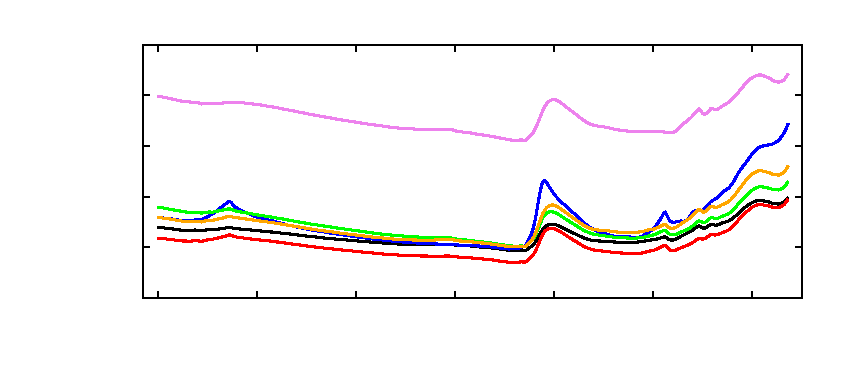
\includegraphics{gp/soil-spec-rnd}}%
    \gplfronttext
  \end{picture}%
\endgroup

			\caption{This figure shows near infrared soil spectra of six randomly chosen soil samples obtained from the used dataframe.}
			\label{fig:soil-spec-rnd}
		\end{figure*}

		The dataframe is made up of $533$ measured soil samples.
		For everyone of them the in section \ref{ssec:soil-parameters} discussed parameters $p_\m{SOC},p_\m{N},\m{pH}$ and the near infrared spectrum are given.
		The soil spectra consists of $319$ wavelengths ranging from $1400\unit{nm}$ to $2672\unit{nm}$ by a step of $4\unit{nm}$.
		The reflectance $\varrho(\lambda)$ of a sample at a given wavelength $\lambda$ is saved as
		\[
			-\lg \varrho(\lambda) = -\frac{\ln \varrho(\lambda)}{\ln 10}
		\]
		Figure \ref{fig:soil-spec-rnd} shows six randomly chosen soil spectra in a diagram.
	
	% subsection measured-data

	\subsection{Statistical Model}
	\label{ssec:statistical-model}
	
		Let $n\in\SN$ be the soil sample count and $k\in\SN$ with $k\leq n$ the number of measured wavelengths.
		$\varrho_i$ shall be defined as soil spectrum of the $i$th sample for every $i\in\SN,i\leq n$.
		$\lambda_j$ is the $j$th measured wavelength for every $j\in\SN,j\leq k$, also called predictor.
		Then according to section \ref{ssec:measured-data} the measured reflectance values are $x_{ij}$ with
		\[
			x_{ij} \define -\lg \varrho_i(\lambda_j)
		\]
		for every $i,j\in\SN,i\leq n,j\leq k$.
		Through the following matrix it is possible to get an easier notation.
		\[
			X \define (x_{ij}) \in \SR^{n\times k}
		\]
		Let $p^\m{(SOC)}_i, p^\m{(N)}_i, \m{pH}_i$ be the measured soil parameters of the $i$th sample for every $i\in\SN,i\leq n$, also known as observables.
		Then we define the $n$-dimensional vectors
		\begin{alignat*}{3}
			p^\m{(SOC)} &\define&&\ \curvb{p^\m{(SOC)}_i} \\
			p^\m{(N)} &\define&&\ \curvb{p^\m{(N)}_i} \\
			\m{pH} &\define&&\ \curvb{\m{pH}_i}
		\end{alignat*}

		The Beer-Lambert law allows us to make assumptions to the relations of soil spectra and soil parameters.
		In section \ref{ssec:nirs} we saw that the logarithmized reflectance can be written as a linear combination of molar concentrations.
		Hence, vice versa it makes sense to assume that an ASF can be represented by a linear combination of logarithmized reflectance values.

		Now let $P^\m{(SOC)},P^\m{(N)}$ be the appropriate random variables to the soil parameters $p^\m{(SOC)}$ and $p^{(N)}$.
		Then with the above assumption the expected values are given by
		\begin{alignat*}{3}
			\expect P^\m{(SOC)} &=&&\ X\beta^\m{(SOC)}_k + \beta^\m{(SOC)}_0 \definedby \mathbb{X}\beta^\m{(SOC)} \\
			\expect P^\m{(N)} &=&&\ X\beta^\m{(N)}_k + \beta^\m{(N)}_0 \definedby \mathbb{X}\beta^\m{(N)}
		\end{alignat*}
		When $\m{PH}$ is the corresponding random variable to $\m{pH}$ we have to perform a correction because $\m{pH}$ is a logarithmized molar concentration.
		It makes sense to model these with the subsequent expected value.
		\[
			\expect \m{PH} = \ln(X)\beta^\m{(pH)}_k + \beta^\m{(pH)}_0 \definedby \mathbb{X}_{\ln}\beta^\m{(pH)}
		\]

		In physics and chemistry it is a common and error-proven method to assume a normal distribution with a certain variance for measuring errors.
		So with the variances $(\sigma^2)^\m{(SOC)},(\sigma^2)^\m{(N)},(\sigma^2)^\m{(pH)}\in(0,\infty)$ our random variables become
		\begin{alignat*}{3}
			P^\m{(SOC)} &\sim&&\ \FN\curvb{\mathbb{X}\beta^\m{(SOC)}, (\sigma^2)^\m{(SOC)}\idmat_n} \\
			P^\m{(N)} &\sim&&\ \FN\curvb{\mathbb{X}\beta^\m{(N)}, (\sigma^2)^\m{(N)}\idmat_n} \\
			\m{PH} &\sim&&\ \FN\curvb{\mathbb{X}_{\ln}\beta^\m{(pH)}, (\sigma^2)^\m{(pH)}\idmat_n}
		\end{alignat*}
	
	% subsection statistical-model

	\subsection{MLR}
	\label{ssec:mlr}
	
		Multiple linear regression (MLR) or multivariate linear regression is a statistical method for estimating parameters that depend on linear independent variables.
		Let $\mathbb{X}\in\SR^{n\times(k+1)}, n,k\in\SN,k<n$ be the design matrix, $\sigma^2\in(0,\infty)$ and $Y$ be the vector of random variables with
		\[
			Y \sim \FN\curvb{\mathbb{X}\beta,\sigma^2\idmat_n}
		\]
		for a certain $\beta\in\SR^{k+1}$
		Then through the maximum-likelihood-method and a small correction we get two best unbiased estimators $\hat{\beta},\hat{\sigma^2}$ for $\beta$ and $\sigma^2$
		\begin{alignat*}{3}
			\hat{\beta}(Y) &=&&\ \inv{\curvb{\transp{\mathbb{X}}\mathbb{X}}}\transp{\mathbb{X}}Y \\
			\hat{\sigma^2}(Y) &=&&\ \frac{1}{n-(k+1)}\norm{Y - \mathbb{X}\hat{\beta}(Y)}^2
		\end{alignat*}
		Now let $y \define (y_i)\in\SR^n$ be a realization of $Y$.
		In this case we define
		\begin{alignat*}{3}
			\hat{y} &\define&&\ \mathbb{X}\hat{\beta}(y) = \mathbb{X}\inv{\curvb{\transp{\mathbb{X}}\mathbb{X}}}\transp{\mathbb{X}}y \\
			\hat{\sigma^2} &\define&&\ \hat{\sigma^2}(y)
		\end{alignat*}
		For more information please refer to [Quelle:Skript,wikipedia].
	
	% subsection mlr

	\subsection{Mallows' $\m{Cp}$}
	\label{ssec:mallows-cp}
	
		According to sections \ref{ssec:statistical-model} and \ref{ssec:mlr} at this time we are using $k+1 = 320$ predictors for our prediction model.
		Estimating Model Parameters with this large amount of predictors tends to overfit the measured data.
		% Quelle: Tutorial, Skript
		So it would be sensible to choose a \enquote{good} subset of predictors
		\[
			M\subset \set[i\in\SN_0,i\leq k]{\lambda_i}
		\]
		where $\lambda_0$ stands for the defined offset.
		Now through $M$ one can define a new design matrix $\mathbb{X}^{(M)}$.
		Applying MLR to this design matrix gives us new estimators
		\begin{alignat*}{3}
			\hat{\beta}^{(M)}(Y) &=&&\ \inv{\curvb{\transp{\mathbb{X}^{(M)}}\mathbb{X}^{(M)}}}\transp{\mathbb{X}^{(M)}}Y \\
			\hat{\sigma^2}^{(M)}(Y) &=&&\ \frac{1}{n-\#M}\norm{Y - \mathbb{X}^{(M)}\hat{\beta}^{(M)}(Y)}^2
		\end{alignat*}
		
		The term \enquote{good} refers to a criterion by which we can define the \enquote{goodness} of $M$.
		Here we will use Mallows' $\m{Cp}$.
		\[
			\m{Cp}^{(M)} \define \frac{1}{\hat{\sigma^2}}\sum_{i=1}^n\curvb{y_i-\hat{y}^{(M)}_i}^2 - n + 2\#M
		\]
		The minimization this value is equivalent to the minimization of the sum of predicted squared errors (SPSE).
	
	% subsection mallows-cp

	\subsection{Simulated Annealing}
	\label{ssec:simulated-annealing}
	
		The set of predictors contains $k=319$ free selectable elements (the constant shall remain).
		Therefore the power set $\s{P}$, the set of possible subsets $M$, contains of $2^{k}=2^{319}$ elements.
		If we want to find a subset $M$ so that for all $N\in\s{P}$ the inequation holds
		\[
			\m{Cp}^{(M)} \leq \m{Cp}^{(N)}
		\]
		we have to calculate $\m{Cp}^{(N)}$ for every $N\in\s{P}$.
		But this is a calculation beyond our current computing power.

		Simulated annealing (SA) is a probabilistic technique for approximating the global optimum of a given function.
		Specifically, it is a metaheuristic to approximate global optimization in a large search space.
		It simulates the slow cooling of a thermodynamic system through random numbers.
		With this algorithm it is possible to find a \enquote{good} local minimum in a short time.
		% Quelle: https://en.wikipedia.org/wiki/Simulated_annealing

		The algorithm works on an arbitrary set, in our case $\s{P}$.
		Let $x_0\in\s{P}$ be the initial set of predictors, $T_0\in(0,\infty)$ be the initial temperature of the system and $i_\m{max}\in\SN$ be the maximal number of time steps.
		Then the algorithm needs certain functions.
		\begin{itemize}
			\item $\func{\m{cost}}{\s{P}}{\SR}$ \\
				Calculates the cost of a given predictor set.
			\item $\func{\m{temp}}{\SR\times\SN^2}{(0,\infty)}$\\
				Calculates the temperature according to the given initial temperature and time steps.
				It is a monotonically decreasing function in the second parameter.
			\item $\func{\m{nbr}}{\s{P}}{\s{P}}$ \\
				Generates a random neighbor of a given predictor set.
			\item $\func{\m{prob}}{\SR^2\times(0,\infty)}{[0,1]}$ \\
				Calculates the probability of changing the current set or state to the neighbor.
			\item $\m{rnd}(0,1)$ \\
				Returns a random number in the interval $[0,1]$.
		\end{itemize}
		The listing shows one variant of the pseudocode of the SA algorithm. 

		\medskip
		\begin{tcolorbox}[colframe=black,colbacktitle=white,coltitle=black, attach boxed title to top center={yshift=-2mm},enhanced, titlerule=0.1pt, boxrule=0.5pt, arc=5pt,title=Listing:\quad SA algorithm]
			\begin{tabbing}
	\qquad\=\qquad\=\qquad\=\qquad\=\kill
	$c_0 = \m{cost}(x_0)$\\
	\\
	\textbf{for} ($i=1$, $i\leq i_\m{max}$) \{\\
		\>$T = \m{temp}(T_0,i,i_\m{max})$\\
		\\
		\>$x_1 = \m{nbr}(x_0)$\\
		\>$c_1 = \m{cost}(x_1)$\\
		\\
		\>\textbf{if} $(\m{prob}(c_0, c_1, T) \geq \m{rnd}(0,1))$ \{\\
			\>\>$x_0 = x_1$\\
			\>\>$c_0 = c_1$\\
		\>\}\\
	\}
\end{tabbing}
		\end{tcolorbox}
		\medskip

	
	% subsection simulated-annealing

	\subsection{Model Validation}
	\label{ssec:model-validation}
	
		% goodness of prediction
	
	% subsection model-validation

% section fundamentals